\documentclass[]{article}
\usepackage{lmodern}
\usepackage{amssymb,amsmath}
\usepackage{ifxetex,ifluatex}
\usepackage{fixltx2e} % provides \textsubscript
\ifnum 0\ifxetex 1\fi\ifluatex 1\fi=0 % if pdftex
  \usepackage[T1]{fontenc}
  \usepackage[utf8]{inputenc}
\else % if luatex or xelatex
  \ifxetex
    \usepackage{mathspec}
  \else
    \usepackage{fontspec}
  \fi
  \defaultfontfeatures{Ligatures=TeX,Scale=MatchLowercase}
\fi
% use upquote if available, for straight quotes in verbatim environments
\IfFileExists{upquote.sty}{\usepackage{upquote}}{}
% use microtype if available
\IfFileExists{microtype.sty}{%
\usepackage{microtype}
\UseMicrotypeSet[protrusion]{basicmath} % disable protrusion for tt fonts
}{}
\usepackage[margin=1in]{geometry}
\usepackage{hyperref}
\hypersetup{unicode=true,
            pdftitle={Lecture 2: Probability models and stochasticity},
            pdfborder={0 0 0},
            breaklinks=true}
\urlstyle{same}  % don't use monospace font for urls
\usepackage{graphicx,grffile}
\makeatletter
\def\maxwidth{\ifdim\Gin@nat@width>\linewidth\linewidth\else\Gin@nat@width\fi}
\def\maxheight{\ifdim\Gin@nat@height>\textheight\textheight\else\Gin@nat@height\fi}
\makeatother
% Scale images if necessary, so that they will not overflow the page
% margins by default, and it is still possible to overwrite the defaults
% using explicit options in \includegraphics[width, height, ...]{}
\setkeys{Gin}{width=\maxwidth,height=\maxheight,keepaspectratio}
\IfFileExists{parskip.sty}{%
\usepackage{parskip}
}{% else
\setlength{\parindent}{0pt}
\setlength{\parskip}{6pt plus 2pt minus 1pt}
}
\setlength{\emergencystretch}{3em}  % prevent overfull lines
\providecommand{\tightlist}{%
  \setlength{\itemsep}{0pt}\setlength{\parskip}{0pt}}
\setcounter{secnumdepth}{0}
% Redefines (sub)paragraphs to behave more like sections
\ifx\paragraph\undefined\else
\let\oldparagraph\paragraph
\renewcommand{\paragraph}[1]{\oldparagraph{#1}\mbox{}}
\fi
\ifx\subparagraph\undefined\else
\let\oldsubparagraph\subparagraph
\renewcommand{\subparagraph}[1]{\oldsubparagraph{#1}\mbox{}}
\fi

%%% Use protect on footnotes to avoid problems with footnotes in titles
\let\rmarkdownfootnote\footnote%
\def\footnote{\protect\rmarkdownfootnote}

%%% Change title format to be more compact
\usepackage{titling}

% Create subtitle command for use in maketitle
\newcommand{\subtitle}[1]{
  \posttitle{
    \begin{center}\large#1\end{center}
    }
}

\setlength{\droptitle}{-2em}

  \title{Lecture 2: Probability models and stochasticity}
    \pretitle{\vspace{\droptitle}\centering\huge}
  \posttitle{\par}
  \subtitle{WILD6900}
  \author{}
    \preauthor{}\postauthor{}
      \predate{\centering\large\emph}
  \postdate{\par}
    \date{updated 2018-11-26}


\begin{document}
\maketitle

\textbf{Warning: The material presented in this lecture is tedious. But
the concepts in this lecture are critical to everything that will follow
in this course. So push through and try your best to understand these
topics. You do not need to be an expert in probability at the end of
this lecture - we will reinforce these concepts over and over again
throughout the semester - but getting the gist now will help you grasp
other topics as we move forward.}

\hypertarget{stochasticity-and-uncertainty-in-ecological-models}{%
\section{Stochasticity and uncertainty in ecological
models}\label{stochasticity-and-uncertainty-in-ecological-models}}

In lecture 1, we learned about the different levels of models we
typically encounter in ecological studies. Recall that for each level,
we differentiated between a deterministic portion of the model \(g()\)
and a stochastic portion \([a|b,c]\). The determinstic portion of the
model contains no uncertainty - given a certain input, it will always
return the same answer.

\emph{Stochastic} processes are different - given an input, the model
will not always return the same answer. So stochastic processes are ones
where the output is uncertain. However, even though stochastic processes
are inherently uncertain, that does not mean they are unpredictable.

We also learned in the last lecture that what makes a model
\emph{Bayesian} is that all unobserved quantity is treated as a random
variable, that is one tha tcan take on different values due to chance.
Each random variable in our models is governed by a probabilty
distribution. Our goal is to use our data to learn about those
distributions. Because probability distributions for the basis of
Bayesian methods, a good understanding of probability is critical to
everything that will follow.

\hypertarget{probability}{%
\section{Probability}\label{probability}}

We said earlier than uncertain events are not necessarily unpredictable.
In most cases, we can summarise how likely each possible value of a
random variable is to occur. This is the essence of \emph{probability}.

\hypertarget{sample-space}{%
\subsection{Sample space}\label{sample-space}}

For any given random variable, we can define the \emph{sample space}
\(S\), which includes all of the possible values the variable can take.
For example, for an single-species occupancy model, \(S\) would be
present or absent. For a model of species abundance, \(S\) would be
\({0,1,2,3,...,\infty}\).

\textbf{insert figure}

For our random process to truly be a probability, the sum of the
probabilities of all must equal 1: \(\sum_{i=1}^n Pr(A_i) = 1\) (if the
outcomes are continous we have to take the intergral instead of the
sum).

As an example, let's imagine an occupancy model in which we want to know
if species \(x\) is present at a given location. We will denote the
occupancy status \(z_x\) and the sample space includes just two possible
values:

\[S_{z_x}=\{0, 1\}\]

\hypertarget{probability-of-single-events}{%
\subsection{Probability of single
events}\label{probability-of-single-events}}

Within the sample space, we can define a smaller polygon \(A\) which
represents one possible outcome. \(A\) is smaller than \(S\) because it
does not contain all possible outcomes, just a subset.

We can define the probability that \(A\) will occur as the area of \(A\)
divided by the area of \(S\).

\[Pr(A) = \frac{area\; of\; A}{area\; of \;S}\]

What is the probability that \(A\) does not occur? It's the area outside
of \(A\):

\[Pr(not \; A) = \frac{area\; of \;S - area\; of\; A}{area\; of \;S} = 1 - \frac{area\; of\; A}{area\; of \;S} = 1 - Pr(A)\]

In our example, let's say that the probability of occupancy for species
\(x\) is \(Pr(z_x = 1) = 0.4\). This means that the probability that the
site in not occupied is \(Pr(z_x = 0) =1-0.4=0.6\).

\hypertarget{probability-of-multiple-events}{%
\subsection{Probability of multiple
events}\label{probability-of-multiple-events}}

Often, we are not interested in the probability of a single event
happening but instead of more than one events. The \emph{joint}
probability refers to the probability that two or more events occur and
is usually denoted \(Pr(A,B)\). Estimating joint probabilities is more
challenging than estimating the probability of single events but is
critical to understanding the logic behind Bayesian methods.

To extend our simple example, let's imagine we are interested in the
occupancy status of two species - \(x\) and \(y\). Our sample space is
now:

\[S_{z_x,z_y} = \{(0,0), (0,1), (1,0), (1,1)\}\]

The question we want to know now is: what is the probability that a site
is occupied by both species, \(Pr(z_x = 1, z_y = 1)\) (which can shorten
to \(Pr(z_x, z_y)\))

The answer to that question depends on the relationship between
\(Pr(z_x)\) and \(Pr(z_y)\)

\hypertarget{conditional-probability}{%
\subsubsection{Conditional probability}\label{conditional-probability}}

In some cases, knowing the status of one random variable tells us
something about the status of another random variable.

Let's say we know that species \(x\) is present, that is \(z_x=1\).
Knowing that \(z_x=1\) does two things:

\begin{enumerate}
\def\labelenumi{\arabic{enumi})}
\item
  It shrinks the possible range of sample space (if \(z_x=1\) occured,
  the remainder of our sample space (in this case \(z_x=0\)) did not
  occur)
\item
  It effectively shrinks the area \(z_y\) - we know that the area of
  \(z_y\) outside of \(z_x\) didn't occur
\end{enumerate}

So the \(Pr(z_y|z_x)\) (read, probability of \(z_y\) conditional on
\(z_x\)) is the area shared by the two events divided by the area of
\(z_y\) (not \(S\)!)

\[Pr(z_y|z_x) = \frac{area\; shared\; by\; z_x\; and\; z_y}{area\; of \;z_x} = \frac{Pr(z_x\; \cap\; z_y)}{Pr(z_x)}\]

\emph{\(\cap\) means ``intersection'' and it is the area shared by both
\(A\) and \(B\)}

likewise,

\[Pr(z_x|z_y) = \frac{Pr(z_x\; \cap\; z_y)}{Pr(z_y)}\]

For conditional events, the joint probability is:

\[Pr(z_y, z_x) = Pr(z_y|z_x)Pr(z_x) = Pr(z_x|z_y)Pr(z_y)\]

\hypertarget{probability-of-independent-events}{%
\subsubsection{Probability of independent
events}\label{probability-of-independent-events}}

In some cases, the probability of one event occuring is
\emph{independent} of whether or not the other event occurs. For
example, the probability of a coin flip being heads is not dependent on
whether or not the previous flip was heads. In our example, the
occupancy of the two species may be totally unrelated so if they occur
together, it happens by complete chance (this maybe unlikely since even
if they don't interact with each other, habitat preferences alone might
lead to non-independence but we'll discuss that in a more detail
shortly). In this case, knowing that \(z_x=1\) gives us no new
information about the probability of \(z_y=1\). Mathmatically, this
means that:

\[Pr(z_y|z_x) = Pr(z_y)\]

and

\[Pr(z_x|z_y) = Pr(z_x)\]

Thus,

\[Pr(z_x,z_y) = Pr(z_x)Pr(z_y)\] Note that this equation \emph{only}
applies to events that are statistically independent.

\hypertarget{disjoint-events}{%
\subsubsection{Disjoint events}\label{disjoint-events}}

A special case of condtional probability is when events are
\emph{disjoint}. In our case, let's say that species \(x\) and species
\(y\) \textbf{never} occur together (maybe they are such fierce
competitors that they will exclude each other from their territories).
In this case, knowing that \(z_x = 1\) means that \(z_y = 0\). In other
words,

\[Pr(z_y|z_x) = Pr(z_x|z_y) = 0\]
\textgreater{}\textgreater{}\textgreater{}\textgreater{}\textgreater{}\textgreater{}\textgreater{}
3db29a4504a4a6f2213b3ea1e250ac09d3b763cc

\textbf{insert figure}

\hypertarget{probability-of-one-event-or-the-other}{%
\subsubsection{Probability of one event or the
other}\label{probability-of-one-event-or-the-other}}

In some cases, we might want to know the probability that one event
\emph{or} the other occurs. For example, what is the probability that
species \(x\) or species \(y\) is present but not both. This is the area
in \(z_x\) and \(z_y\) not including the area of overlap:

\[Pr(z_x \cup z_y) = Pr(z_x) + Pr(z_y) - Pr(z_x,z_y)\]

When \(z_x\) and \(z_y\) are independent,

\[Pr(z_x \cup z_y) = Pr(z_x) + Pr(z_y) - Pr(z_x)Pr(z_y)\]

If they are conditional,

\[Pr(z_x \cup z_y) = Pr(z_x) + Pr(z_y) - Pr(z_x|z_y)Pr(z_y) = Pr(z_x) + Pr(z_y) - Pr(z_y|z_x)Pr(z_x)\]

If they are disjoint,

\[Pr(z_x \cup z_y) = Pr(z_x) + Pr(z_y)\]

\hypertarget{marginal-probability}{%
\subsection{Marginal probability}\label{marginal-probability}}

Now let's imagine that our occupancy model includes the effect of 3
different habitats on the occupancy probability of species \(x\), so:

\[Pr(z_x|H_i) = \frac{Pr(z_x \cap H_i)}{Pr(H_i)}\]

What is the overall probability that species \(x\) occurs regardless of
habitat type? That is, \(Pr(z_x)\)?

In this case, we \emph{marginalize} over the different habitat types by
summing the conditional probabilities weighted by probability of each
\(H_i\):

\[Pr(z_x) = \sum_{i=1}^3 Pr(z_x|H_i)Pr(H_i)\]

Think of this as a weighted average - the probability that \(z_x=1\) in
each habitat type weighted by the probability that each habitat type
occurrs.

\hypertarget{complex-joint-probabilities}{%
\section{Complex joint
probabilities}\label{complex-joint-probabilities}}

\hypertarget{bayesian-networks}{%
\subsection{Bayesian networks}\label{bayesian-networks}}

Bayesian networks graphically display the dependences among random
variables.

Random variables are \emph{nodes}. Arrows point from \emph{parents} to
\emph{children}

Networks allow us to factor comples joint probabilities into a series of
more simple conditional probabilities

\hypertarget{factoring-joint-probabilities}{%
\subsection{Factoring joint
probabilities}\label{factoring-joint-probabilities}}

We already saw that:

\[Pr(A, B) = Pr(A|B)Pr(B)\]

We can generalize this to more than two events, which we will call
\(z_1, z_2,...,z_n\):

\[Pr(z_1, z_2,...,z_n) = Pr(z_n|z_{n-1},...,z_1)...Pr(z_3|z_2, z_1)Pr(z_2|z_1)Pr(z_1)\]

\hypertarget{properties-of-probability-distributions}{%
\section{Properties of probability
distributions}\label{properties-of-probability-distributions}}

Because all unobserved quantities are treated as random variables
governed by probability distributions, using and understanding Bayesian
methods requires understanding probability distributions.

As ecologists, there are a number of very common probability
distributions that we encounter and use regularly (normal, Poisson,
binomial, gamma, etc.). We are not going to go over the properties of
each of these distributions in lecture today. Instead, I will talk about
specific distributions as they come up in examples.

Even though I will discuss specific distributions as they come up, I
highly recommend you read the chapter of \emph{Hobbs \& Hooten} on
probability functions to familiarize yourself with the distributions
we'll use throughout the semester. If you don't have that book, just
google each distribution and read the wikipedia page.

\hypertarget{discrete-vs.continuous-distributions}{%
\subsection{Discrete vs.~continuous
distributions}\label{discrete-vs.continuous-distributions}}

Before discussing the properties of probability distributions, we must
first distinguish between discrete and continuous random variables.
\emph{Continuous} random variables are those that can take on an
infinite number of values on a specific interval. The most familiar
continous distribution is the normal, which allows any value from
\(-\infty\) to \(\infty\). Other ranges are possible. For example, a
random variable could take any value between \(0\) and \(1\) or any
value \textgreater{} \(0\). Aside from the normal distribution, common
continuous distributions include the uniform, gamma, beta, and
exponential.

\emph{Discrete} random variables are those that take on distinct values,
usually (but not always) integers. In ecology, we usually encounter
discrete variables in the form of counts (the number of individuals can
only be postive integers, you can't have 4.234 individuals) or
categories (alive vs.~dead, present in location A vs.~B vs.~C). Common
probability distributions for discrete variables include Poisson,
binomial, negative binomial, and multinomial.

We will encounter all of these distributions throughout the semester.

\hypertarget{probability-functions}{%
\subsection{Probability functions}\label{probability-functions}}

Very often we want to know the probability that a random variable will
take a specific value \(z\). Answering this question requires the use of
probability functions, which we will denote \([z]\). So probability
functions tell us \([z]=Pr(z)\).

Probability functions differ between \emph{continuous} and
\emph{discrete} distributions so we will discuss these separately.
Probability functions for discrete variables are a little easier to
understand so we will start with them.

\hypertarget{probability-mass-functions}{%
\subsubsection{Probability mass
functions}\label{probability-mass-functions}}

For \emph{discrete} random variables, the probability that the variable
will take a specific value \(z\) is defined by the \emph{probability
mass function}.

All pmf's share two properties:

\[0 \leq [z] \leq 1\] \[\sum_{z \in S}[z]=1\]

where \(S\) is the set of all \(z\) for which \([z] > 0\) (the range of
possible values of \(z\)).

As an example, let's assume a random variable that follows a Poisson
distribution. Poisson random variables can take any integer value
\textgreater{} 0 (\(0, 1, 2,...\)). This could be the number of
individuals at a site or the number of seeds produced by a flower.

The shape of the Poisson distribution is determined by 1 parameter
called \(\lambda\) (greek lambda). We'll discuss this more in a minute
but \(\lambda\) is the expected value (the most likely value) of a
random variable generated from the Poisson distribution. So larger
\(\lambda\) means larger values of the variable.

Let's say that for our example distribution \(\lambda = 10\). What is
the probability that \(z\) will equal exactly 10? Or 8? Or 15? In R,
probabitity mass is estimating using the \texttt{dpois()} function (or
the equivalent for other discrete distributions), which takes two
arguments: the value we are interested in estimating the probability of
(\(z\)) and the expected value of our distribution (\(\lambda\)):
\texttt{dpois(x\ =\ 10,\ lambda\ =\ 10)}. R will let us put in a vector
of values so we can also do the following to estimate the probability of
all values from 0 to 25:
\texttt{dpois(x\ =\ seq(0,\ 25),\ lambda\ =\ 10)}

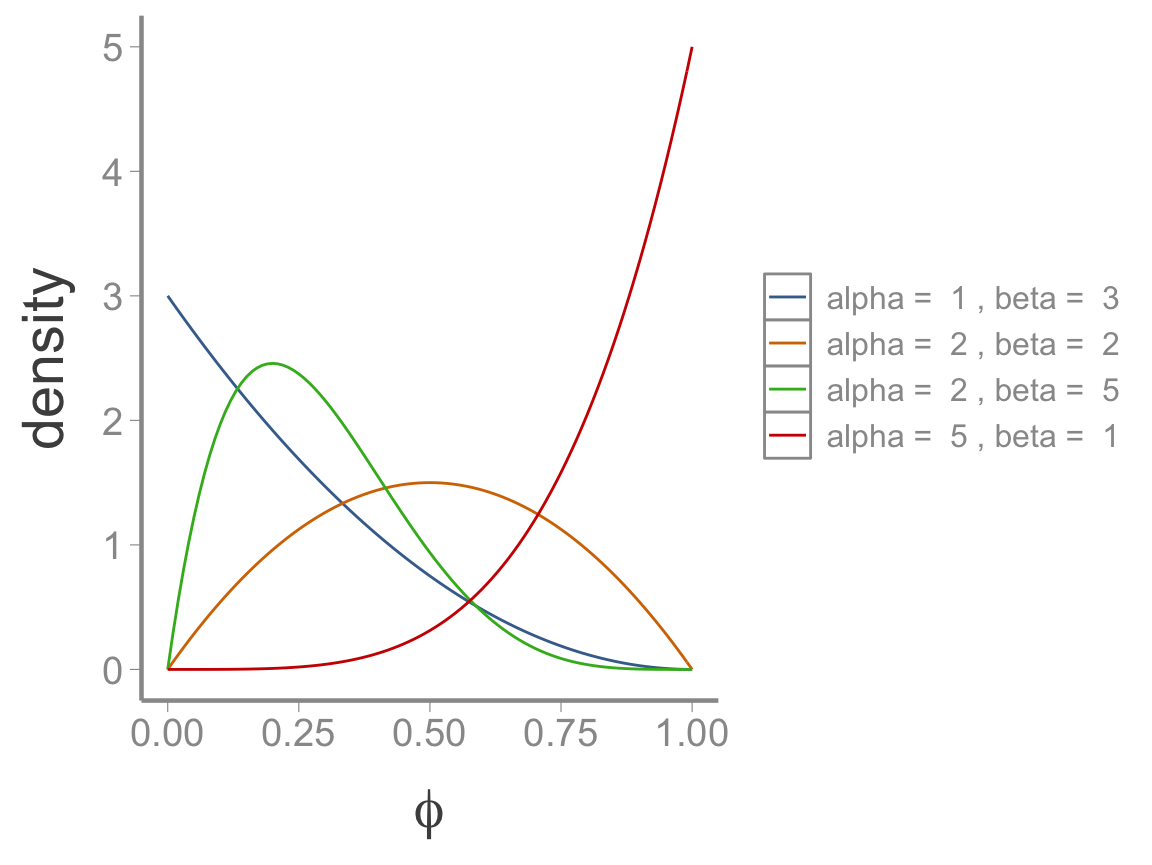
\includegraphics{lecture2-notes_files/figure-latex/unnamed-chunk-1-1.pdf}

\hypertarget{probability-density-functions}{%
\subsubsection{Probability density
functions}\label{probability-density-functions}}

Probability mass functions provide the probability that a discrete
random variable takes on a specific value \(z\). For continuous
variables, estimating probabilities is a little trickier. This is
because \(Pr(z) = 0\) for any specific value \(z\). Why is this?

Let's look at the probability distribution for a normal random variable
with mean \(=0\) and standard deviation \(=3\):

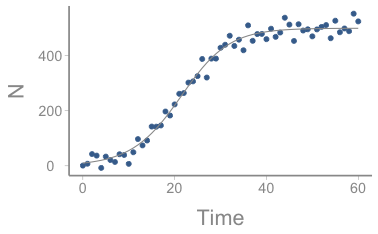
\includegraphics{lecture2-notes_files/figure-latex/unnamed-chunk-2-1.pdf}

The \emph{probability density} is the area under the curve for an
interval between \(a\) and \(b\), which we'll call \(\Delta_z\)
(\(=a-b\)).. For example, the shaded area below shows the probability
density \(Pr(-2 \leq z \leq -1\) for our normal distribution:

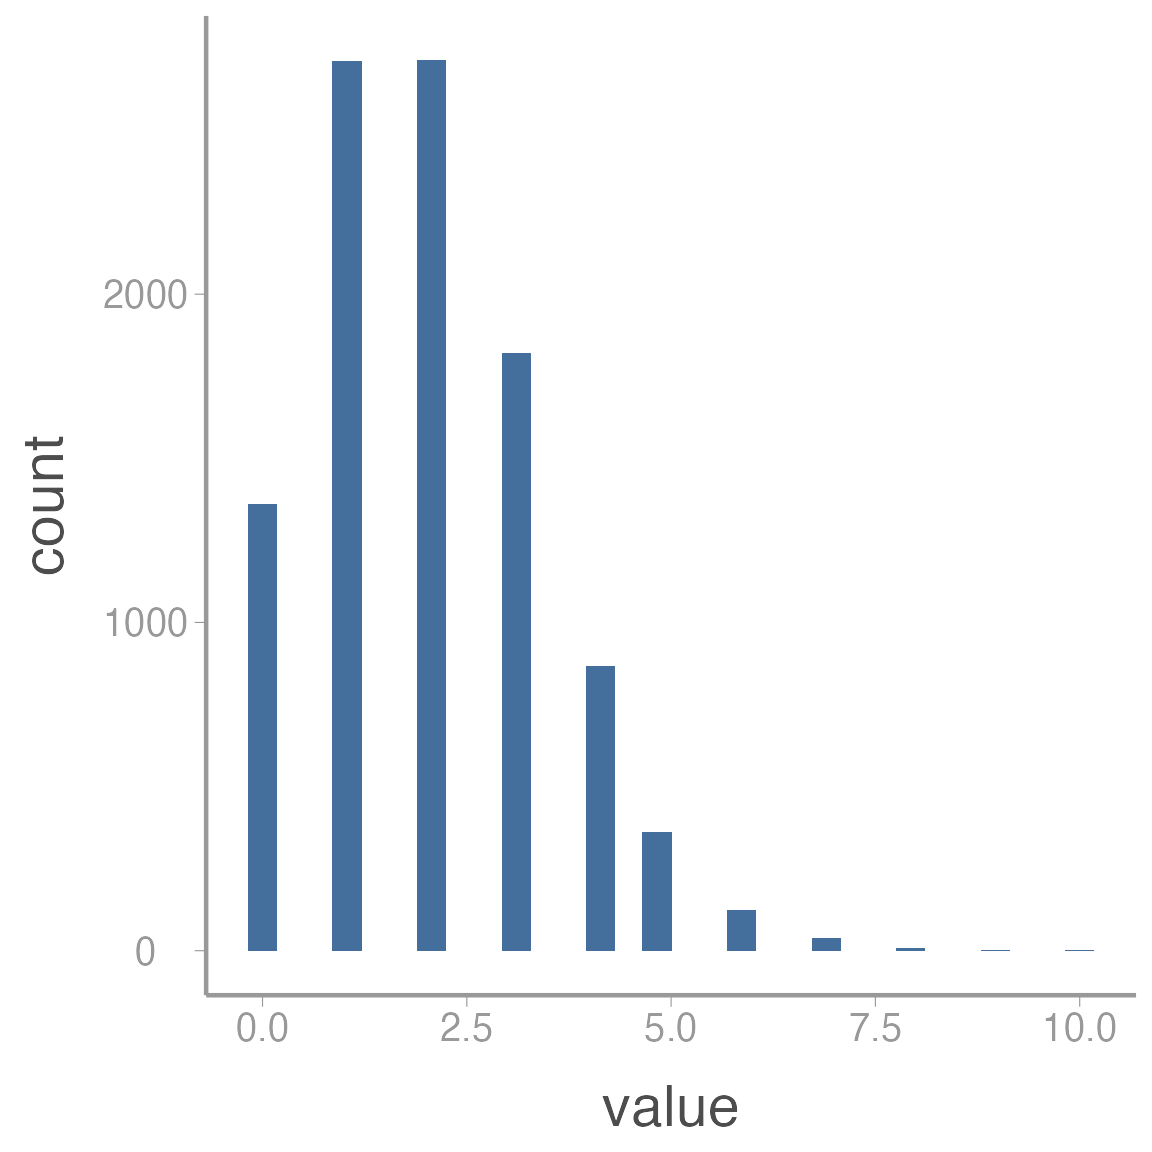
\includegraphics{lecture2-notes_files/figure-latex/unnamed-chunk-3-1.pdf}

This area can be approximated by multiplying the width times the
(average) height of the rectangle:

\[Pr(a \leq z \leq b) \approx \Delta_z [(a + b)/2]\]

By making the range \(\Delta_z =a-b\) smaller and smaller, we get closer
to \(Pr(z)\):

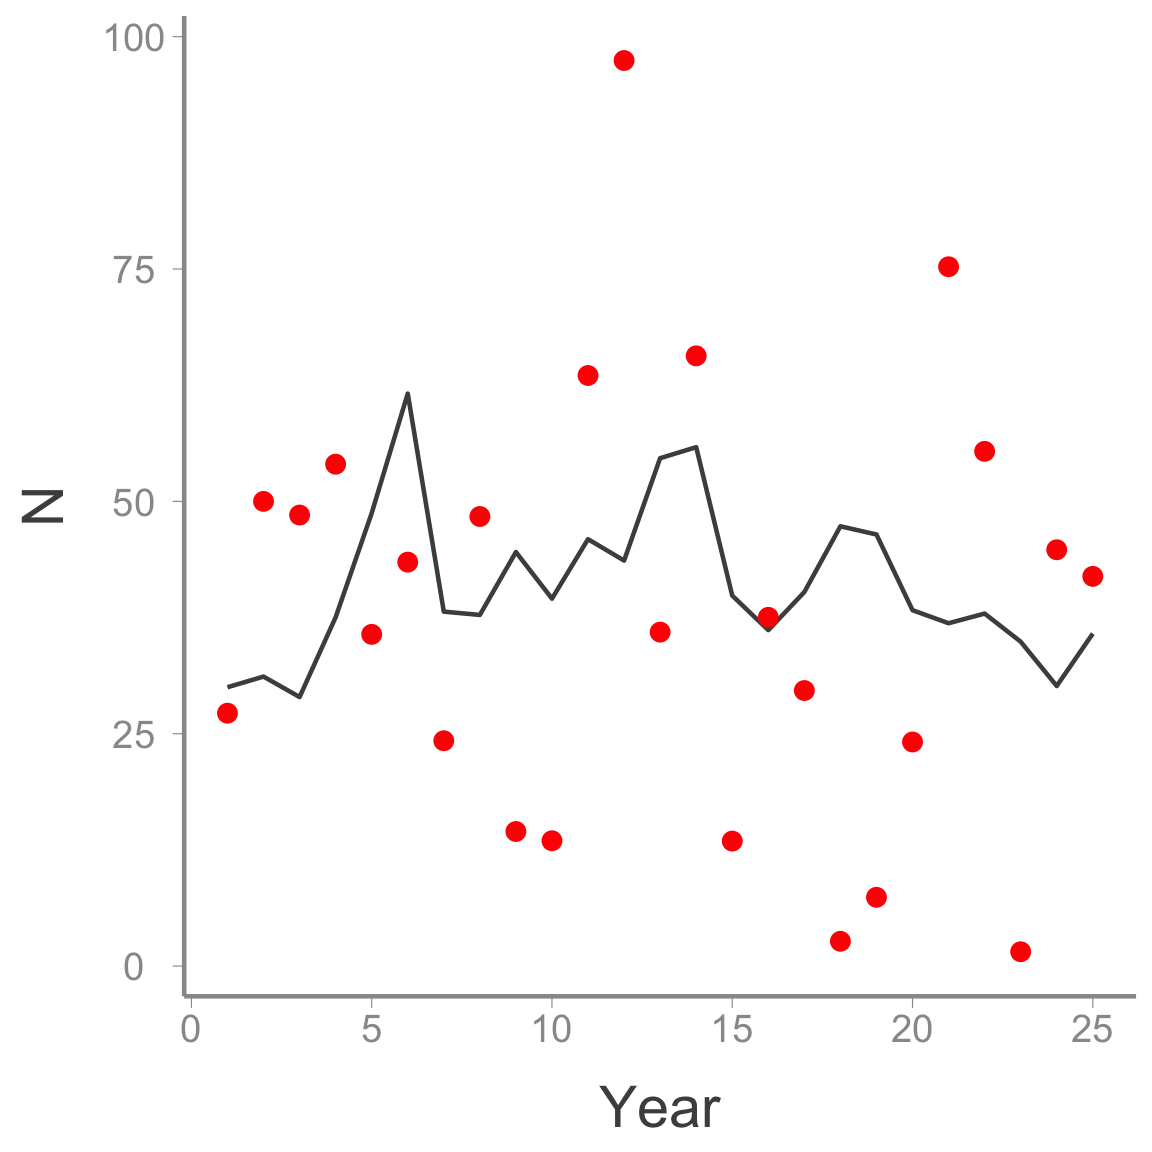
\includegraphics{lecture2-notes_files/figure-latex/unnamed-chunk-4-1.pdf}

However, at \(z\), \(\Delta_z =0\), thus \([z] = 0\). However, we can
use calculus to estimate the height of the line (\([z]\)) as
\(\Delta_z\) approaches 0.

So for continuous random variables, the \emph{probability density} of
\(z\) is the area under the curve between \(a \leq z \leq b\) as
\(\Delta_z\) approaches zero. Estimating probability density in R is the
same as for discrete variables: \texttt{dnorm()}. Now you know why the
function starts with \texttt{d}!

\hypertarget{moments}{%
\subsection{Moments}\label{moments}}

Every probability distribution we will use in the course can be
described by its \emph{moments}. We will mostly use the first and second
moments of each distribution so this is what we will focus on here.

\hypertarget{expected-value-i.e.-the-mean}{%
\subsubsection{Expected value (i.e., the
mean)}\label{expected-value-i.e.-the-mean}}

The first moment of a distribution describes its central tendency
(denoted \(\mu\)) or \emph{expected value} (denoted \(E(z)\). This is
the most probable value of \(z\). Think of this as a weighted average -
the mean of all possible values of \(z\) weighted by the probability
mass or density of each value (\([z]\)). For discrete variables, the
first moment can be calculated as

\[\mu = E(z) = \sum_{z \in S} z[z]\]

For continous variables, we need to use an integral instead of a sum:

\[\mu = E(z) = \int_{-\infty}^{\infty} z[z]dz\]

\hypertarget{variance}{%
\subsubsection{Variance}\label{variance}}

The second moment of a distribution describes the \emph{variance} - that
is, the spread of the distribution around its mean. In other words, on
average how far is a random value drawn from the distribution from the
mean of the distribution. For discrete variables, variance can be
estimated as the weighted average of the squared difference (squared to
prevent negative values) between each value \(z\) and the mean \(\mu\)
of the distribution:

\[\sigma^2 = E((z - \mu)^2) = \sum_{z \in S} (z - \mu)^2[z]\]

and for continous variables:

\[\sigma^2 = E((z - \mu)^2) = \int_{-\infty}^{\infty} (z - \mu)^2[z]dz\]

\hypertarget{exercise-estimating-moments-using-monte-carlo-integration}{%
\subsubsection{\texorpdfstring{Exercise: Estimating moments using
\emph{Monte Carlo
integration}}{Exercise: Estimating moments using Monte Carlo integration}}\label{exercise-estimating-moments-using-monte-carlo-integration}}

One way to estimate moments is by simulating a large number of values
from a probability distribution and then using these samples to
calculate the first and second moments. This is a useful approach to
understand because it is very similar to how we learn about parameter
distributions in Bayesian analyses. It's also very easy to do in
\texttt{R} using the \texttt{r} class of functions (e.g.,
\texttt{rnorm()}, \texttt{rpois()}, etc.). These functions generate
specified number of random draws (\texttt{r} for random) from a given
probability distribution.

For example, let's estimate the first and second moments of a gamma
distribution. The gamma distribution is continuous probability
distribution that produces non-negative random variables. The shape of
the distribution is governed by two parameters, \(\alpha\) (refered to
as the shape) and \(\beta\) (referred to as the rate or sometimes the
scale). Both \alpha\$ and \(\beta\) must be \(>0\). In \texttt{R}, we
can generate and visualize a large number (e.g., 10000) random draws
from the gamma distribution using the following code:

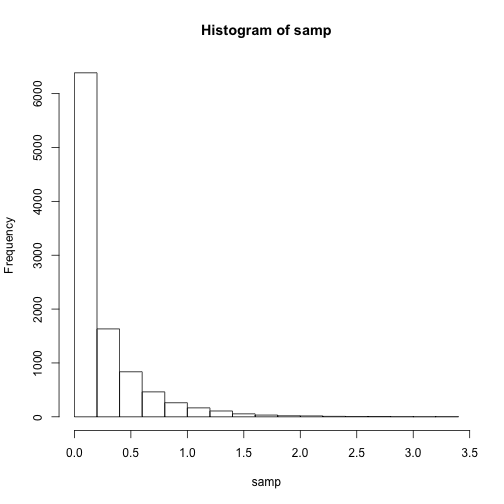
\includegraphics{lecture2-notes_files/figure-latex/unnamed-chunk-5-1.pdf}

Now let's use these sample to estimate the first moment (the mean) and
the second moment (the variance) of these samples. We estimate the first
moment by taking the arithmetic mean of our samples
(\(\frac{1}{n}{\sum_{i=1}^{n}z_i}\)) and the variance as
(\(\frac{1}{n}{\sum_{i=1}^{n}(z_i-\mu)^2}\)):

How close are these values to the true moments? For the gamma
distribution: \(\mu = \frac{\alpha}{\beta}\) and
\(\sigma^2 = \frac{\alpha}{\beta^1}\). For our distribution:

\begin{verbatim}
## [1] 0.2449
\end{verbatim}

\begin{verbatim}
## [1] 0.25
\end{verbatim}

\begin{verbatim}
## [1] 0.1247
\end{verbatim}

\begin{verbatim}
## [1] 0.125
\end{verbatim}

Pretty close. Try this on your own - simulate data from a Poisson
distribution and see if the moments you estimate from the sample are
close to the true moments. \textbf{hint} - the poisson distribution has
a single parameter \(\lambda\), which is both the mean and the variance
of the distribution. Change both \(\lambda\) and \(n\). \emph{Does
varying these values change how well your sample estimates the moments?}

\textbf{Question} - in the above simulations, we use the arithmetic mean
to estimate the first moment of the distribution. But in the definition
of the moment, we defined the mean as the weighted average of the
\(z\)'s. Why don't we have to take the weighted average of our sample?

\hypertarget{moment-matching}{%
\subsubsection{Moment matching}\label{moment-matching}}

For the normal distribution, it is relatively easy to understand moments
because the parameters of the distribution (mean and standard deviation)
\emph{are} the first and second moments. In addition to being intuitive,
the normal distribution has an interesting (though maybe not obvious)
property - you can change the first moment (the mean) without changing
the second moment (the variance)

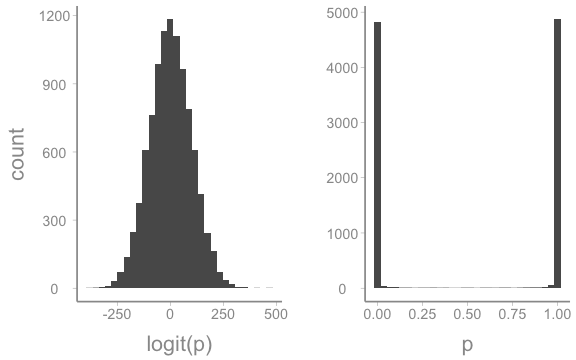
\includegraphics{lecture2-notes_files/figure-latex/unnamed-chunk-8-1.pdf}

This is not true of all probability distributions. For example, the beta
distribution is a continuous distribution with values between 0 and 1.
This makes it useful for modeling random variables that are
probabilities (e.g., detection probability in an occupancy model). The
shape of the Beta distribution is governed by two parameters \(\alpha\)
and \(\beta\) and its first and second moments are:

\[\mu = \frac{\alpha}{\alpha + \beta}\]

\[\sigma^2 = \frac{\alpha\beta}{(\alpha + \beta)^2 (\alpha + \beta + 1)}\]
If you know \(\alpha\) and \(\beta\), it's easy to estimate the mean and
variance using these formulas. But what is I tell you that species \(x\)
has an estimated mean detection probability of 0.3 and variance of 0.1.
How do you translate those into the relevant beta distribution? We need
another set of equations:

\[\alpha = \bigg(\frac{1-\mu}{\sigma^2}- \frac{1}{\mu} \bigg)\mu^2\]

\[\beta = \alpha \bigg(\frac{1}{\mu}-1\bigg)\]

For our ouccupancy probability, that means:

\begin{verbatim}
## [1] 0.33
\end{verbatim}

\begin{verbatim}
## [1] 0.77
\end{verbatim}

Let's use our simulation method to check that our estimates are correct:

\begin{verbatim}
## [1] 0.302
\end{verbatim}

\begin{verbatim}
## [1] 0.09922
\end{verbatim}

This process of converting between parameters and moments is called
\emph{moment matching}. It's a very important process becasue often we
have the mean and variance of distributions but need to convert those
summaries into the parameters of the underlying distribution (if this is
not obvious right now, don't worry. You'll see why later in the semester
as we work through examples). Of course, this does not mean you need to
memorize the moment equations - that's what google is for.


\end{document}
